\section{Introduction}\label{sec:intro}
Inductors in second order systems can be replaced by amplifiers and capacitors.
Fig.~\ref{fig:schematic} shows an active second order system with a gain of $G = 1 + {R_a \over R_b}$.

\begin{figure}[tbph]
	\centering
	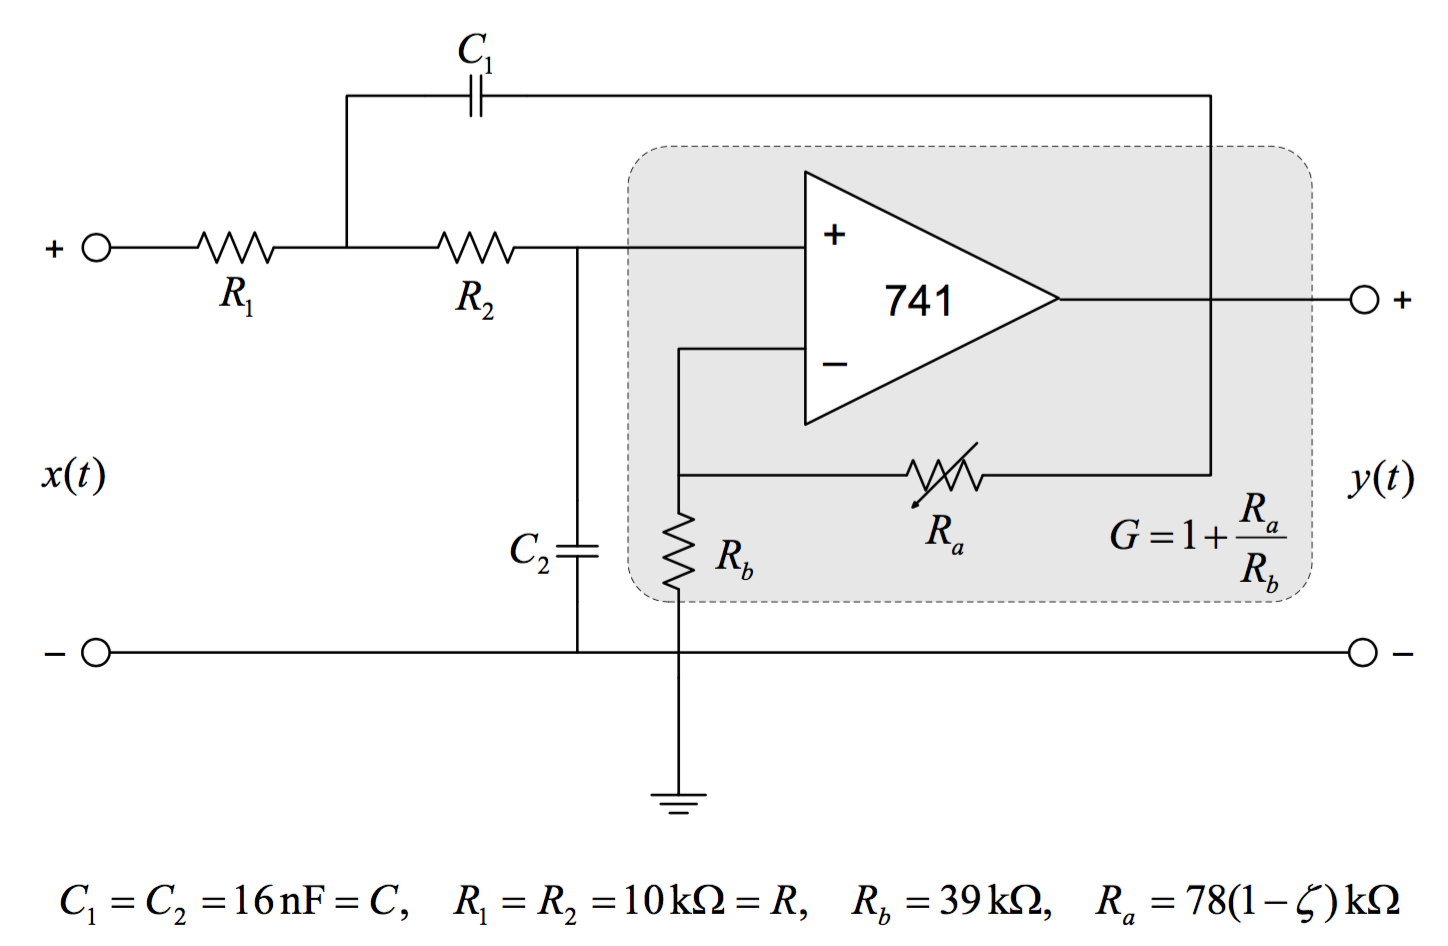
\includegraphics[width=0.7\linewidth]{graphics/schematic}
	\caption{Active realization of a second order system}
	\label{fig:schematic}
\end{figure}

The transfer function of this system is:
\begin{equation}\label{eqn:tf}
	H(s) = { G \omega_0^2 \over s^2 + 2\zeta\omega_0 s + \omega_0^2 }
\end{equation}
where 
\begin{equation}\label{eqn:freq}
	\omega_0 = {1 \over RC}
\end{equation}and
\begin{equation}\label{eqn:damping}
	\zeta = 1 - {R_a \over 2R_b}.
\end{equation}

When the unit step function is applied to Fig.~\ref{fig:schematic} it will produce an output similar to Fig.~\ref{fig:overshoot_expected}.

\begin{figure}[tbph]
	\centering
	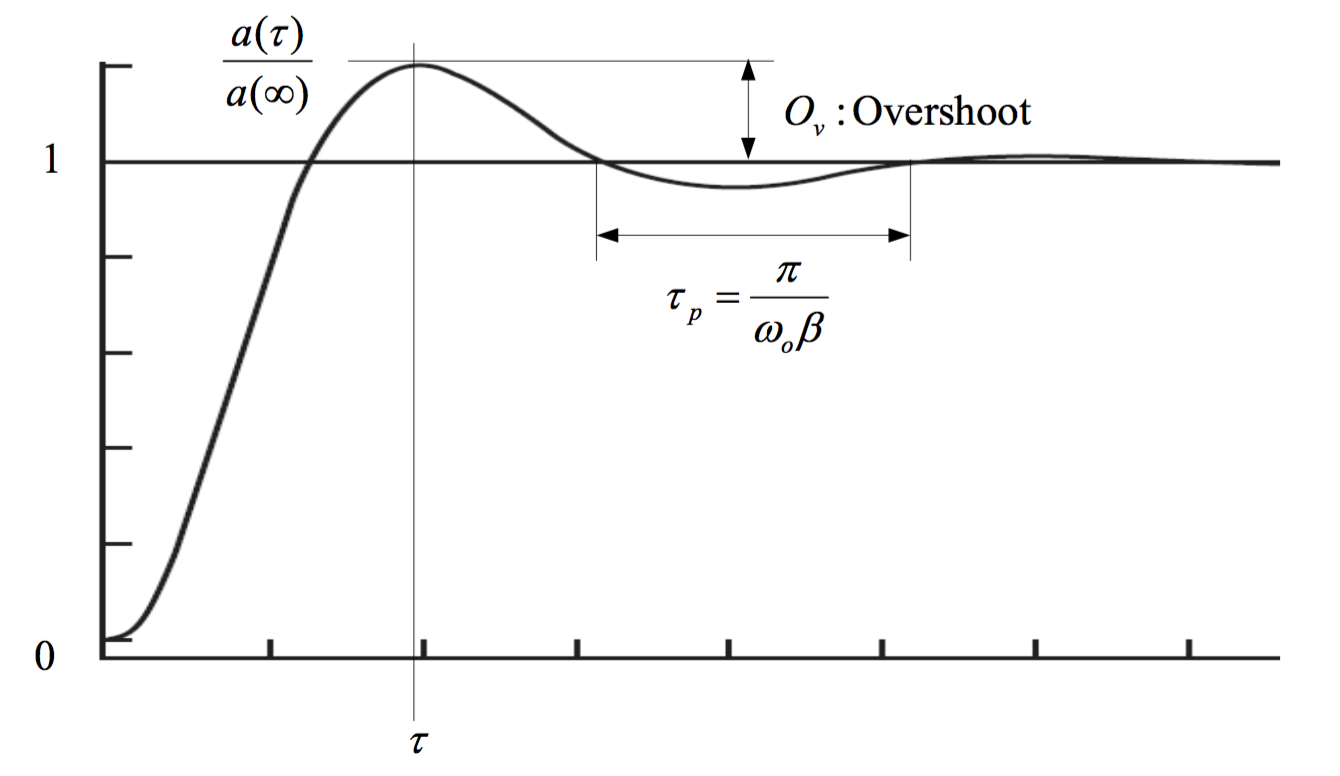
\includegraphics[width=0.7\linewidth]{graphics/overshoot_expected}
	\caption{Step response of second order system}
	\label{fig:overshoot_expected}
\end{figure}

The system parameters $\zeta$ and $\omega_0$ can be obtained from this graph since:
\begin{align}
	O_v &= \exp \left( { -\zeta\pi \over \beta } \right) \label{eqn:overshoot} \\
	T_p &= { \pi \over \omega_0\beta }. \label{eqn:period}
\end{align}

$O_v$ can be obtained from Fig.~\ref{fig:overshoot_expected} as:
\begin{equation*}
	O_v = {V_{peak} - V_{steady} \over V_{steady}}.
\end{equation*}
